\documentclass[]{article}
\usepackage{lmodern}
\usepackage{amssymb,amsmath}
\usepackage{ifxetex,ifluatex}
\usepackage{fixltx2e} % provides \textsubscript
\ifnum 0\ifxetex 1\fi\ifluatex 1\fi=0 % if pdftex
  \usepackage[T1]{fontenc}
  \usepackage[utf8]{inputenc}
\else % if luatex or xelatex
  \ifxetex
    \usepackage{mathspec}
  \else
    \usepackage{fontspec}
  \fi
  \defaultfontfeatures{Ligatures=TeX,Scale=MatchLowercase}
\fi
% use upquote if available, for straight quotes in verbatim environments
\IfFileExists{upquote.sty}{\usepackage{upquote}}{}
% use microtype if available
\IfFileExists{microtype.sty}{%
\usepackage{microtype}
\UseMicrotypeSet[protrusion]{basicmath} % disable protrusion for tt fonts
}{}
\usepackage[margin=1in]{geometry}
\usepackage{hyperref}
\hypersetup{unicode=true,
            pdfborder={0 0 0},
            breaklinks=true}
\urlstyle{same}  % don't use monospace font for urls
\usepackage{color}
\usepackage{fancyvrb}
\newcommand{\VerbBar}{|}
\newcommand{\VERB}{\Verb[commandchars=\\\{\}]}
\DefineVerbatimEnvironment{Highlighting}{Verbatim}{commandchars=\\\{\}}
% Add ',fontsize=\small' for more characters per line
\usepackage{framed}
\definecolor{shadecolor}{RGB}{248,248,248}
\newenvironment{Shaded}{\begin{snugshade}}{\end{snugshade}}
\newcommand{\KeywordTok}[1]{\textcolor[rgb]{0.13,0.29,0.53}{\textbf{#1}}}
\newcommand{\DataTypeTok}[1]{\textcolor[rgb]{0.13,0.29,0.53}{#1}}
\newcommand{\DecValTok}[1]{\textcolor[rgb]{0.00,0.00,0.81}{#1}}
\newcommand{\BaseNTok}[1]{\textcolor[rgb]{0.00,0.00,0.81}{#1}}
\newcommand{\FloatTok}[1]{\textcolor[rgb]{0.00,0.00,0.81}{#1}}
\newcommand{\ConstantTok}[1]{\textcolor[rgb]{0.00,0.00,0.00}{#1}}
\newcommand{\CharTok}[1]{\textcolor[rgb]{0.31,0.60,0.02}{#1}}
\newcommand{\SpecialCharTok}[1]{\textcolor[rgb]{0.00,0.00,0.00}{#1}}
\newcommand{\StringTok}[1]{\textcolor[rgb]{0.31,0.60,0.02}{#1}}
\newcommand{\VerbatimStringTok}[1]{\textcolor[rgb]{0.31,0.60,0.02}{#1}}
\newcommand{\SpecialStringTok}[1]{\textcolor[rgb]{0.31,0.60,0.02}{#1}}
\newcommand{\ImportTok}[1]{#1}
\newcommand{\CommentTok}[1]{\textcolor[rgb]{0.56,0.35,0.01}{\textit{#1}}}
\newcommand{\DocumentationTok}[1]{\textcolor[rgb]{0.56,0.35,0.01}{\textbf{\textit{#1}}}}
\newcommand{\AnnotationTok}[1]{\textcolor[rgb]{0.56,0.35,0.01}{\textbf{\textit{#1}}}}
\newcommand{\CommentVarTok}[1]{\textcolor[rgb]{0.56,0.35,0.01}{\textbf{\textit{#1}}}}
\newcommand{\OtherTok}[1]{\textcolor[rgb]{0.56,0.35,0.01}{#1}}
\newcommand{\FunctionTok}[1]{\textcolor[rgb]{0.00,0.00,0.00}{#1}}
\newcommand{\VariableTok}[1]{\textcolor[rgb]{0.00,0.00,0.00}{#1}}
\newcommand{\ControlFlowTok}[1]{\textcolor[rgb]{0.13,0.29,0.53}{\textbf{#1}}}
\newcommand{\OperatorTok}[1]{\textcolor[rgb]{0.81,0.36,0.00}{\textbf{#1}}}
\newcommand{\BuiltInTok}[1]{#1}
\newcommand{\ExtensionTok}[1]{#1}
\newcommand{\PreprocessorTok}[1]{\textcolor[rgb]{0.56,0.35,0.01}{\textit{#1}}}
\newcommand{\AttributeTok}[1]{\textcolor[rgb]{0.77,0.63,0.00}{#1}}
\newcommand{\RegionMarkerTok}[1]{#1}
\newcommand{\InformationTok}[1]{\textcolor[rgb]{0.56,0.35,0.01}{\textbf{\textit{#1}}}}
\newcommand{\WarningTok}[1]{\textcolor[rgb]{0.56,0.35,0.01}{\textbf{\textit{#1}}}}
\newcommand{\AlertTok}[1]{\textcolor[rgb]{0.94,0.16,0.16}{#1}}
\newcommand{\ErrorTok}[1]{\textcolor[rgb]{0.64,0.00,0.00}{\textbf{#1}}}
\newcommand{\NormalTok}[1]{#1}
\usepackage{graphicx,grffile}
\makeatletter
\def\maxwidth{\ifdim\Gin@nat@width>\linewidth\linewidth\else\Gin@nat@width\fi}
\def\maxheight{\ifdim\Gin@nat@height>\textheight\textheight\else\Gin@nat@height\fi}
\makeatother
% Scale images if necessary, so that they will not overflow the page
% margins by default, and it is still possible to overwrite the defaults
% using explicit options in \includegraphics[width, height, ...]{}
\setkeys{Gin}{width=\maxwidth,height=\maxheight,keepaspectratio}
\IfFileExists{parskip.sty}{%
\usepackage{parskip}
}{% else
\setlength{\parindent}{0pt}
\setlength{\parskip}{6pt plus 2pt minus 1pt}
}
\setlength{\emergencystretch}{3em}  % prevent overfull lines
\providecommand{\tightlist}{%
  \setlength{\itemsep}{0pt}\setlength{\parskip}{0pt}}
\setcounter{secnumdepth}{0}
% Redefines (sub)paragraphs to behave more like sections
\ifx\paragraph\undefined\else
\let\oldparagraph\paragraph
\renewcommand{\paragraph}[1]{\oldparagraph{#1}\mbox{}}
\fi
\ifx\subparagraph\undefined\else
\let\oldsubparagraph\subparagraph
\renewcommand{\subparagraph}[1]{\oldsubparagraph{#1}\mbox{}}
\fi

%%% Use protect on footnotes to avoid problems with footnotes in titles
\let\rmarkdownfootnote\footnote%
\def\footnote{\protect\rmarkdownfootnote}

%%% Change title format to be more compact
\usepackage{titling}

% Create subtitle command for use in maketitle
\newcommand{\subtitle}[1]{
  \posttitle{
    \begin{center}\large#1\end{center}
    }
}

\setlength{\droptitle}{-2em}

  \title{}
    \pretitle{\vspace{\droptitle}}
  \posttitle{}
    \author{}
    \preauthor{}\postauthor{}
    \date{}
    \predate{}\postdate{}
  

\begin{document}

\begin{Shaded}
\begin{Highlighting}[]
\NormalTok{knitr}\OperatorTok{::}\NormalTok{opts_chunk}\OperatorTok{$}\KeywordTok{set}\NormalTok{(}\DataTypeTok{echo =} \OtherTok{TRUE}\NormalTok{)}
\NormalTok{nsims <-}\StringTok{ }\DecValTok{100000} \CommentTok{#set number of simulations}
\KeywordTok{require}\NormalTok{(mvtnorm, }\DataTypeTok{quietly =} \OtherTok{TRUE}\NormalTok{)}
\KeywordTok{require}\NormalTok{(MASS, }\DataTypeTok{quietly =} \OtherTok{TRUE}\NormalTok{)}
\KeywordTok{require}\NormalTok{(afex, }\DataTypeTok{quietly =} \OtherTok{TRUE}\NormalTok{)}
\KeywordTok{require}\NormalTok{(emmeans, }\DataTypeTok{quietly =} \OtherTok{TRUE}\NormalTok{)}
\KeywordTok{require}\NormalTok{(ggplot2, }\DataTypeTok{quietly =} \OtherTok{TRUE}\NormalTok{)}
\KeywordTok{require}\NormalTok{(gridExtra, }\DataTypeTok{quietly =} \OtherTok{TRUE}\NormalTok{)}
\KeywordTok{require}\NormalTok{(reshape2, }\DataTypeTok{quietly =} \OtherTok{TRUE}\NormalTok{)}
\KeywordTok{require}\NormalTok{(pwr, }\DataTypeTok{quietly =} \OtherTok{TRUE}\NormalTok{)}

\CommentTok{# Install functions from GitHub by running the code below:}
\KeywordTok{source}\NormalTok{(}\StringTok{"https://raw.githubusercontent.com/Lakens/ANOVA_power_simulation/master/ANOVA_design.R"}\NormalTok{)}
\KeywordTok{source}\NormalTok{(}\StringTok{"https://raw.githubusercontent.com/Lakens/ANOVA_power_simulation/master/ANOVA_power.R"}\NormalTok{)}
\KeywordTok{source}\NormalTok{(}\StringTok{"https://raw.githubusercontent.com/Lakens/ANOVA_power_simulation/master/mu_from_ES.R"}\NormalTok{)}
\end{Highlighting}
\end{Shaded}

\subsection{Example of Power in Repeated Measures
ANOVA}\label{example-of-power-in-repeated-measures-anova}

In a repeated measures design multiple observations are collected from
the same participants. In the simplest case, where there are two
repeated observations, a repeated measures ANOVA equals a dependent or
paired \emph{t}-test. The difference compared to a between subject
design is that repeated measures can be correlated, and in psychology,
they often are. Let's first explore the impact of this correlation on
the power of a repeated measures ANOVA.

\subsection{Two conditions, medium effect
size}\label{two-conditions-medium-effect-size}

To illustrate the effect of correated observations, we start by
simulating data for a medium effect size for a dependent (or paired, or
within-subject) \emph{t}-test. Let's first look at G*power. If we want
to perform an a-priori power analysis, we are asked to fill in the
effect size dz. As Cohen (1988) writes, ``The Z subscript is used to
emphasize the fact that our raw score unit is no longer X or Y, but Z'',
where Z are the difference scores of X-Y.

\begin{figure}
\centering
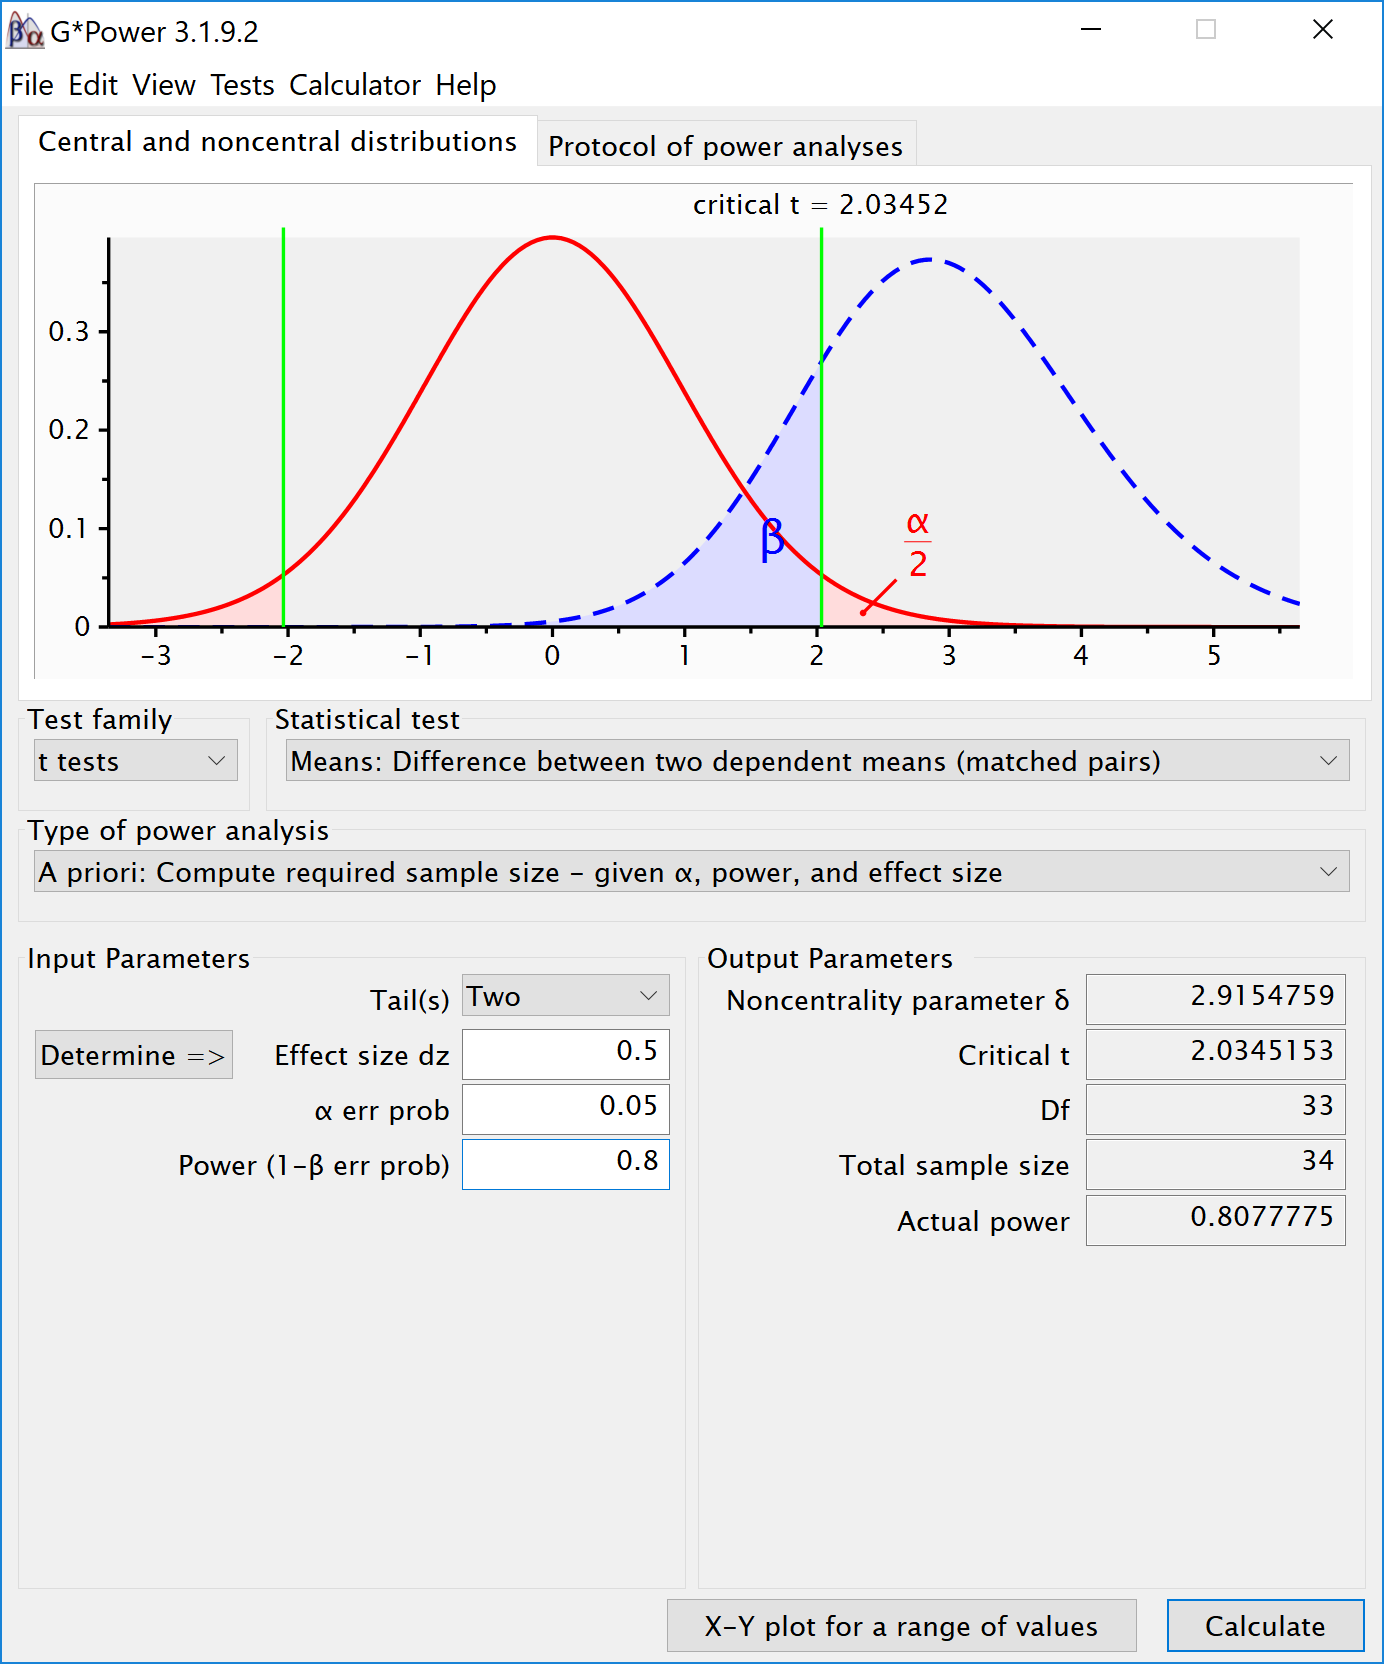
\includegraphics{screenshots/gpower_9.png}
\caption{}
\end{figure}

Within designs can have greater power to detect differences than between
designs because the values are correlated, and a within design requires
less participants because each participant provides multiple
observations. One difference between an independent \emph{t}-test and a
dependent \emph{t}-test is that an independent \emph{t}-test has 2(n-1)
degrees of freedom, while a dependent \emph{t}-test has (n-1) degrees of
freedom. The sample size needed in a two-group within-design (NW)
relative to the sample needed in two-group between-designs (NB),
assuming normal distributions, and ignoring the difference in degrees of
freedom between the two types of tests, is (from Maxwell \& Delaney,
2004, p.~561, formula 45):

\(N_{W}=\frac{N_{B}(1-\rho)}{2}\)

The division by 2 in the equation is due to the fact that in a
two-condition within design every participant provides two data-points.
The extent to which this reduces the sample size compared to a
between-subject design depends on the correlation (\emph{r}) between the
two dependent variables, as indicated by the 1-r part of the equation.
If the correlation is 0, a within-subject design needs half as many
participants as a between-subject design (e.g., 64 instead 128
participants), simply because every participants provides 2 datapoints.
The higher the correlation, the larger the relative benefit of within
designs, and whenever the correlation is negative (up to -1) the
relative benefit disappears.

Whereas in an independent \emph{t}-test the two observations are
uncorrelated, in a within design the observations are correlated. This
has an effect on the standard deviation of the difference scores. In
turn, because the standardized effect size is the mean difference
divided by the standard deviation of the difference scores, the
correlation has an effect on the standardized mean difference in a
within design, Cohen's dz. The relation, as Cohen (1988, formula 2.3.7)
explains, is:

\(\sigma_{z}=\sigma\sqrt{2(1-\rho)}\)

Therefore, the relation between dz and d is \(\sqrt{2(1-\rho)}\). As
Cohen (1988) writes: ``In other words, a given difference between
population means for matched (dependent) samples is standardized by a
value which is \(\sqrt{2(1-\rho)}\) as large as would be the case were
they independent. If we enter a correlation of 0.5 in the formula, we
get \(\sqrt{2(0.5)}=1\). In other words, when the correlation is 0.5, d
= dz. When there is a strong correlation between dependent variables,
for example r = 0.9, we get \(d=d_{z}\sqrt{2(1-0.9)}\), and a dz of 1
would be a d = 0.45. Reversely, \(d_{z}=\frac{d}{\sqrt{2(1-r)}}\), so
with a r = 0.9, a d of 1 would be a dz = 2.24. Some consider this
increase in dz compared to d when observations are strongly correlated
an 'inflation'when estimating effect sizes, but since the reduction in
the standard deviation of the difference scores due to the correlation
makes it easier to distinguish signal from noise in a hypothesis test,
it leads to a clear power benefit.

\begin{Shaded}
\begin{Highlighting}[]
\CommentTok{# Check sample size formula Maxwell}
\CommentTok{# Power is pretty similar with n/2, same d (assuming r = 0.5). }
\CommentTok{# Small differences due to df = 2(n-1) vs df = n-1}
\KeywordTok{pwr.t.test}\NormalTok{(}\DataTypeTok{d =} \FloatTok{0.05}\NormalTok{,}
           \DataTypeTok{n =} \KeywordTok{c}\NormalTok{(}\DecValTok{2000}\NormalTok{, }\DecValTok{4000}\NormalTok{, }\DecValTok{8000}\NormalTok{),}
           \DataTypeTok{sig.level =} \FloatTok{0.05}\NormalTok{,}
           \DataTypeTok{type =} \StringTok{"two.sample"}\NormalTok{,}
           \DataTypeTok{alternative =} \StringTok{"two.sided"}\NormalTok{)}
\end{Highlighting}
\end{Shaded}

\begin{verbatim}
## 
##      Two-sample t test power calculation 
## 
##               n = 2000, 4000, 8000
##               d = 0.05
##       sig.level = 0.05
##           power = 0.3524674, 0.6086764, 0.8853424
##     alternative = two.sided
## 
## NOTE: n is number in *each* group
\end{verbatim}

\begin{Shaded}
\begin{Highlighting}[]
\KeywordTok{pwr.t.test}\NormalTok{(}\DataTypeTok{d =} \FloatTok{0.05}\NormalTok{,}
           \DataTypeTok{n =} \KeywordTok{c}\NormalTok{(}\DecValTok{1000}\NormalTok{, }\DecValTok{2000}\NormalTok{, }\DecValTok{4000}\NormalTok{),}
           \DataTypeTok{sig.level =} \FloatTok{0.05}\NormalTok{,}
           \DataTypeTok{type =} \StringTok{"paired"}\NormalTok{,}
           \DataTypeTok{alternative =} \StringTok{"two.sided"}\NormalTok{)}
\end{Highlighting}
\end{Shaded}

\begin{verbatim}
## 
##      Paired t test power calculation 
## 
##               n = 1000, 2000, 4000
##               d = 0.05
##       sig.level = 0.05
##           power = 0.3520450, 0.6083669, 0.8852320
##     alternative = two.sided
## 
## NOTE: n is number of *pairs*
\end{verbatim}

There is no equivalent fz for Cohen's f for a within subject ANOVA. For
two groups, we can directly compute Cohen's f from Cohen's d for two
groups, as Cohen (1988) describes, because f = 1/2d. For a d = 0.5, f =
0.25. In Gpower we can run a 2 group within-subject power analysis for
ANOVA. We plan for 80\% power, and reproduce the anaysis above for the
dependent \emph{t}-test. This works because the correlation is set to
0.5, when d = dz, and thus the transformation of f=1/2d works.

\begin{figure}
\centering
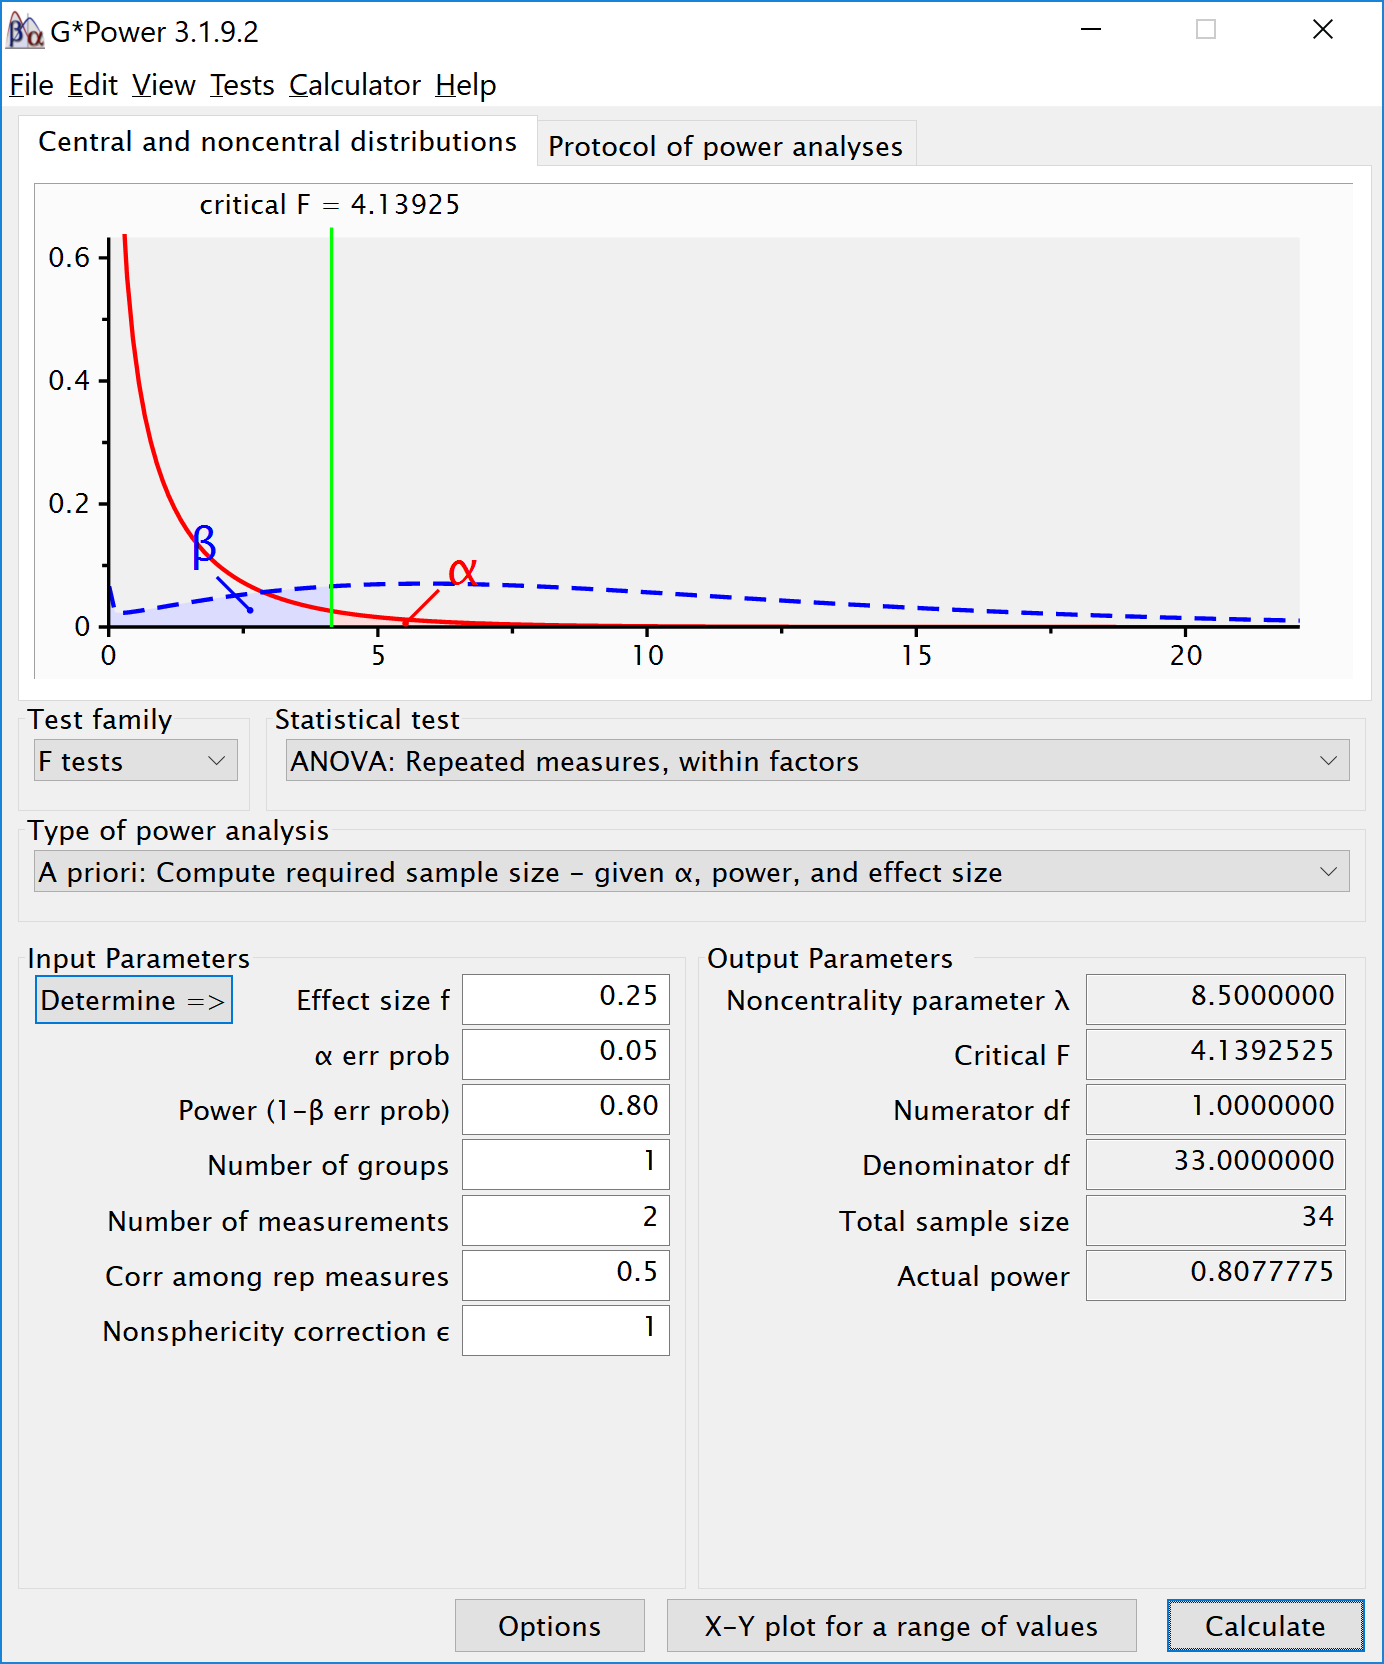
\includegraphics{screenshots/gpower_1.png}
\caption{}
\end{figure}

If we change the correlation to 0.7 and keep all other settings the
same, the repeated measure a-priori power analysis yields a sample of
21. The correlation increases the power for the test.

\begin{figure}
\centering
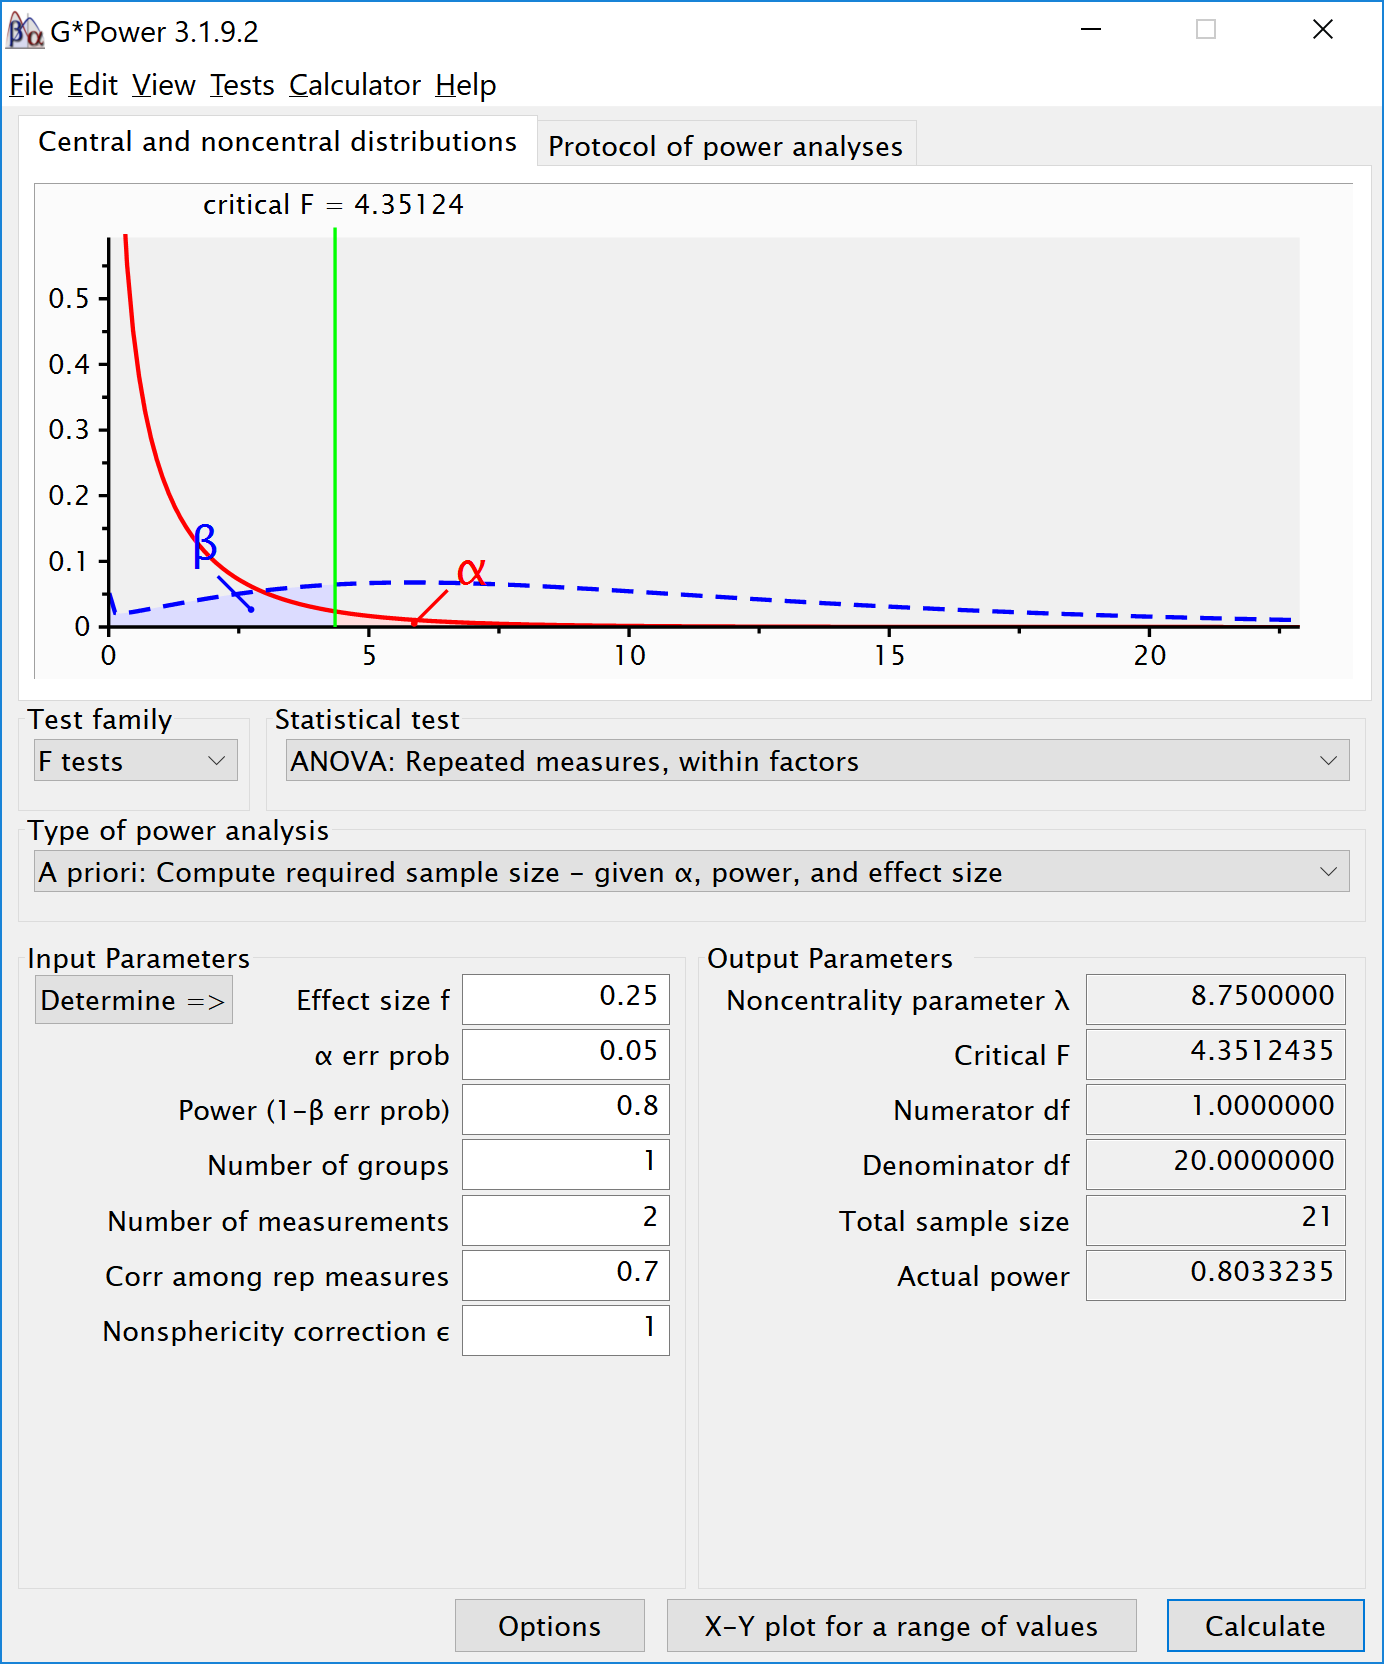
\includegraphics{screenshots/gpower_11.png}
\caption{}
\end{figure}

To reproduce this analysis in Gpower with a dependent \emph{t}-test we
need to change dz following the formula above,
\(d_{z}=\frac{0.5}{\sqrt{2(1-0.7)}}\), which yields dz = 0.6454972. If
we enter this value in Gpower for an a-priori power analysis, we get the
exact same results (as we should, since an repeated measures ANOVA with
2 groups equals a dependent \emph{t}-test). This example illustrates
that the correlation between dependent variables always factors into a
power analysis, both for a dependent \emph{t}-test, and for a repeated
measures ANOVA. Because a dependent \emph{t}-test uses dz the
correlation might be less visible, but given the relation between d and
dz, the correlation is always taken into account and can greatly improve
power for within designs compared to between designs.

\begin{figure}
\centering
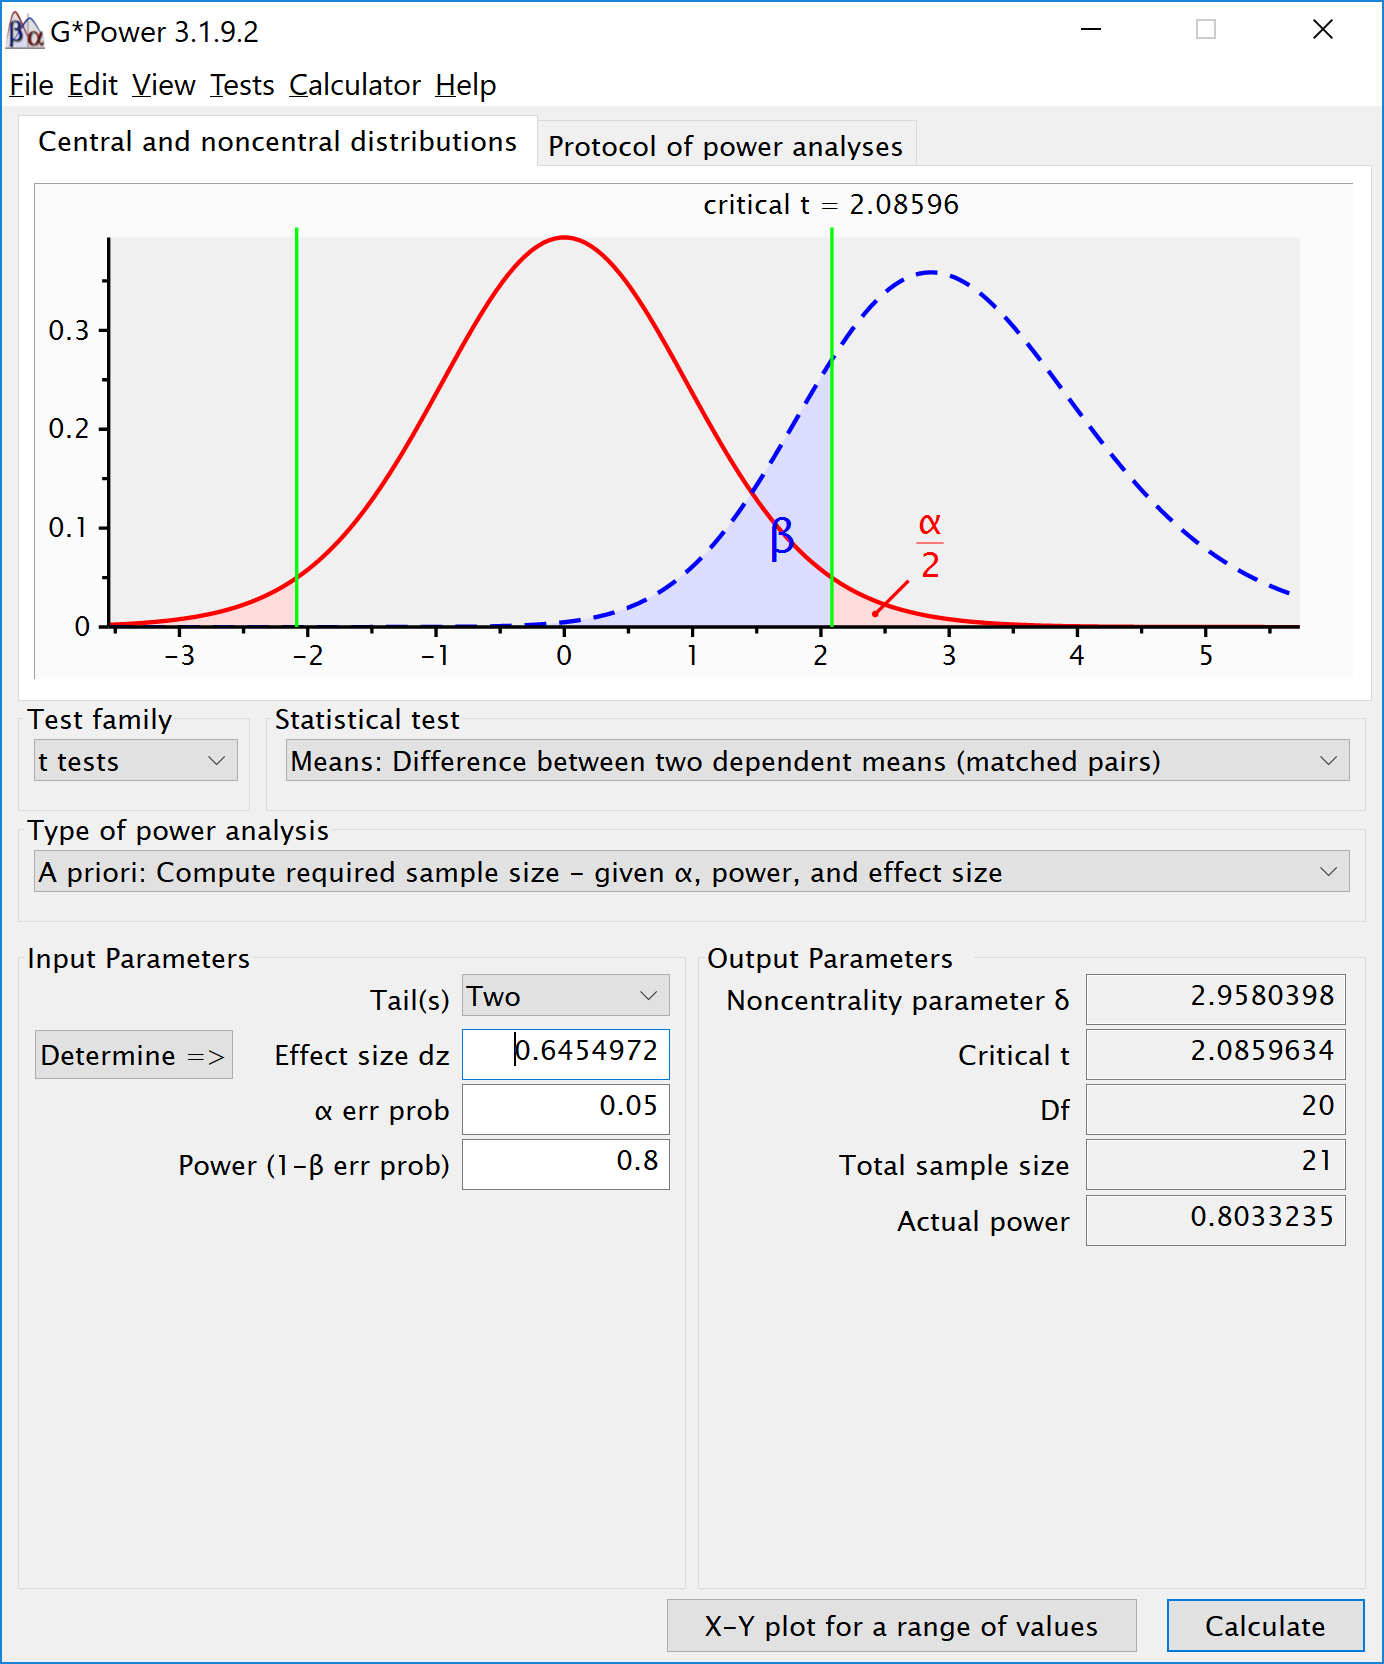
\includegraphics{screenshots/gpower_10.png}
\caption{}
\end{figure}

We can perform both these power analyses using simuations as well. We
set groups to 2 for the simulation, n = 34 (which should give 80.777
power, according to the g*power program), a correlation among repeated
measures of 0.5, and an alpha of 0.05. In this case, we simulate data
with means -0.25 and 0.25, and set the sd to 1. This means we have a
mean difference of 0.5, and a Cohen's d of 0.5/1 = 0.5. In the first
example, we set the correlation to 0.5, and the result should be 80.77\%
power, and an effect size estimate of 0.5 for the simple effect. We also
calculate partial eta-squared for the ANOVA, which equals
\(\frac{f^2}{f^2+1}\), or 0.05882353.

\begin{Shaded}
\begin{Highlighting}[]
\NormalTok{K <-}\StringTok{ }\DecValTok{2}
\NormalTok{n <-}\StringTok{ }\DecValTok{34}
\NormalTok{sd <-}\StringTok{ }\DecValTok{1}
\NormalTok{r <-}\StringTok{ }\FloatTok{0.5}
\NormalTok{alpha =}\StringTok{ }\FloatTok{0.05}
\NormalTok{f <-}\StringTok{ }\FloatTok{0.25}
\NormalTok{f2 <-}\StringTok{ }\NormalTok{f}\OperatorTok{^}\DecValTok{2}
\NormalTok{ES <-}\StringTok{ }\NormalTok{f2}\OperatorTok{/}\NormalTok{(f2}\OperatorTok{+}\DecValTok{1}\NormalTok{)}
\NormalTok{ES}
\end{Highlighting}
\end{Shaded}

\begin{verbatim}
## [1] 0.05882353
\end{verbatim}

\begin{Shaded}
\begin{Highlighting}[]
\NormalTok{mu <-}\StringTok{ }\KeywordTok{mu_from_ES}\NormalTok{(}\DataTypeTok{K =}\NormalTok{ K, }\DataTypeTok{ES =}\NormalTok{ ES)}

\NormalTok{string =}\StringTok{ }\KeywordTok{paste}\NormalTok{(K,}\StringTok{"w"}\NormalTok{,}\DataTypeTok{sep=}\StringTok{""}\NormalTok{)}
\NormalTok{labelnames <-}\StringTok{ }\KeywordTok{c}\NormalTok{(}\StringTok{"speed"}\NormalTok{, }\StringTok{"fast"}\NormalTok{, }\StringTok{"slow"}\NormalTok{)}

\NormalTok{design_result <-}\StringTok{ }\KeywordTok{ANOVA_design}\NormalTok{(}\DataTypeTok{string =}\NormalTok{ string,}
                   \DataTypeTok{n =}\NormalTok{ n, }
                   \DataTypeTok{mu =}\NormalTok{ mu, }
                   \DataTypeTok{sd =}\NormalTok{ sd, }
                   \DataTypeTok{r =}\NormalTok{ r, }
                   \DataTypeTok{labelnames =}\NormalTok{ labelnames)}
\end{Highlighting}
\end{Shaded}

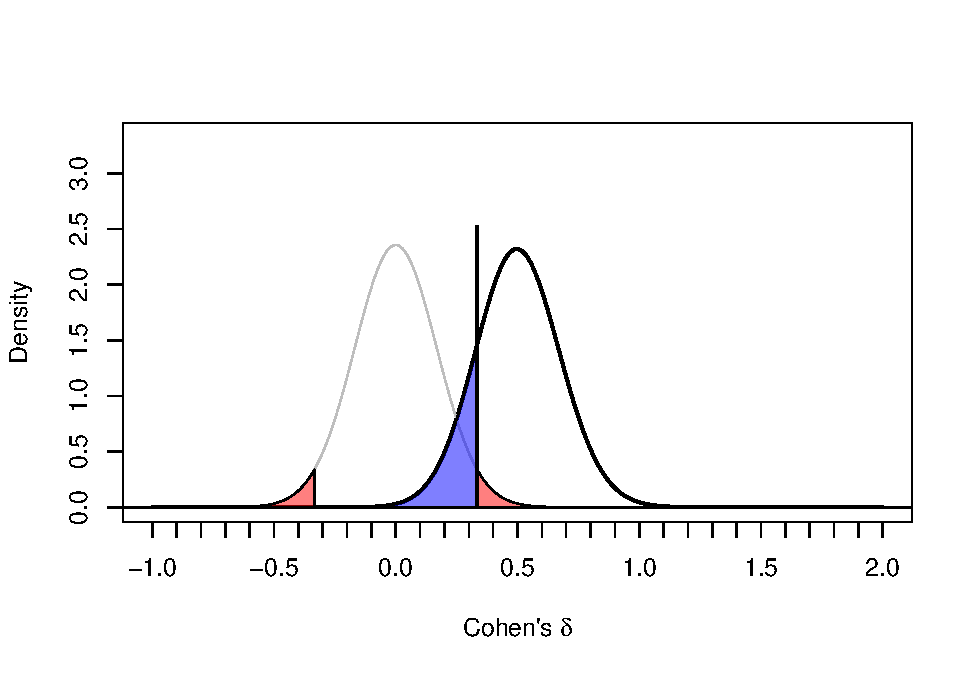
\includegraphics{2.1_validation_power_within_2x1_files/figure-latex/unnamed-chunk-2-1.pdf}

\begin{Shaded}
\begin{Highlighting}[]
\NormalTok{alpha_level <-}\StringTok{ }\FloatTok{0.05}

\KeywordTok{ANOVA_power}\NormalTok{(design_result, }\DataTypeTok{nsims =}\NormalTok{ nsims)}
\end{Highlighting}
\end{Shaded}

\begin{verbatim}
## Power and Effect sizes for ANOVA tests
##              power effect size
## anova_speed 80.966      0.2078
## 
## Power and Effect sizes for contrasts
##                          power effect size
## p_speed_fast_speed_slow 80.966      0.5121
\end{verbatim}

The results of the simulation are indeed very close to 80.777\%. Note
that the simulation calculates Cohen's dz effect sizes for paired
comparisons - which here given the correlation of 0.5 is also 0.5 for a
medium effect size.

We should see a larger dz if we increase the correlation, keeping the
sample size the same, following the example in Gpower above. We repeat
the simulation, and the only difference is a correlation between
dependent variables of 0.7. This should yield an effect size dz =
0.6454972.

\begin{Shaded}
\begin{Highlighting}[]
\NormalTok{K <-}\StringTok{ }\DecValTok{2}
\NormalTok{n <-}\StringTok{ }\DecValTok{21}
\NormalTok{sd <-}\StringTok{ }\DecValTok{1}
\NormalTok{r <-}\StringTok{ }\FloatTok{0.7}
\NormalTok{alpha =}\StringTok{ }\FloatTok{0.05}
\NormalTok{f <-}\StringTok{ }\FloatTok{0.25}
\NormalTok{f2 <-}\StringTok{ }\NormalTok{f}\OperatorTok{^}\DecValTok{2}
\NormalTok{ES <-}\StringTok{ }\NormalTok{f2}\OperatorTok{/}\NormalTok{(f2}\OperatorTok{+}\DecValTok{1}\NormalTok{)}
\NormalTok{ES}
\end{Highlighting}
\end{Shaded}

\begin{verbatim}
## [1] 0.05882353
\end{verbatim}

\begin{Shaded}
\begin{Highlighting}[]
\NormalTok{mu <-}\StringTok{ }\KeywordTok{mu_from_ES}\NormalTok{(}\DataTypeTok{K =}\NormalTok{ K, }\DataTypeTok{ES =}\NormalTok{ ES)}

\NormalTok{string =}\StringTok{ }\KeywordTok{paste}\NormalTok{(K,}\StringTok{"w"}\NormalTok{,}\DataTypeTok{sep=}\StringTok{""}\NormalTok{)}
\NormalTok{labelnames <-}\StringTok{ }\KeywordTok{c}\NormalTok{(}\StringTok{"speed"}\NormalTok{, }\StringTok{"fast"}\NormalTok{, }\StringTok{"slow"}\NormalTok{)}

\NormalTok{design_result <-}\StringTok{ }\KeywordTok{ANOVA_design}\NormalTok{(}\DataTypeTok{string =}\NormalTok{ string,}
                   \DataTypeTok{n =}\NormalTok{ n, }
                   \DataTypeTok{mu =}\NormalTok{ mu, }
                   \DataTypeTok{sd =}\NormalTok{ sd, }
                   \DataTypeTok{r =}\NormalTok{ r, }
                   \DataTypeTok{labelnames =}\NormalTok{ labelnames)}
\end{Highlighting}
\end{Shaded}

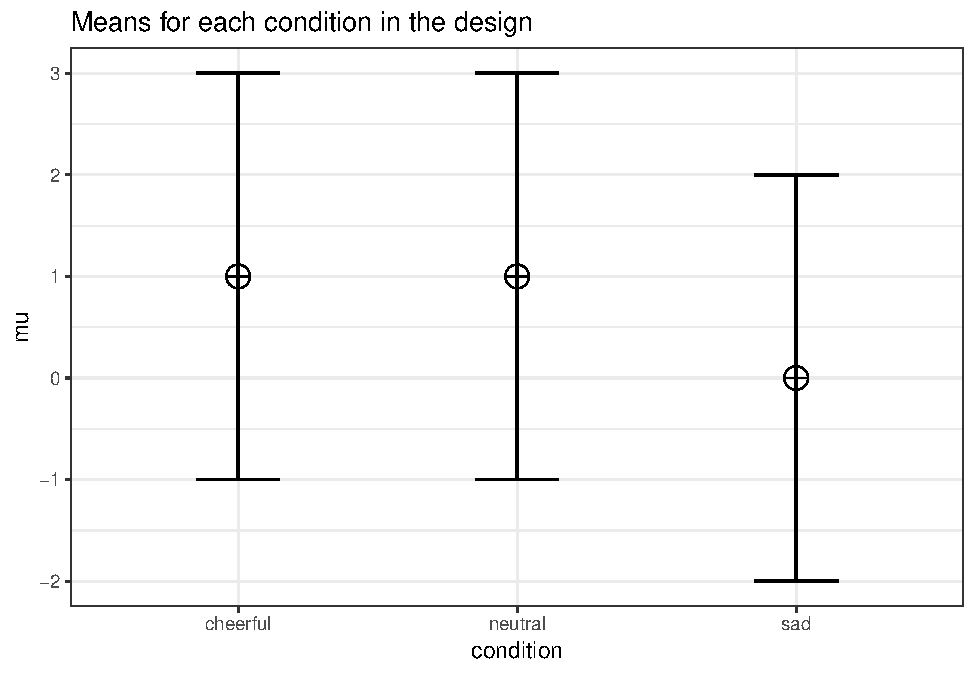
\includegraphics{2.1_validation_power_within_2x1_files/figure-latex/unnamed-chunk-3-1.pdf}

\begin{Shaded}
\begin{Highlighting}[]
\NormalTok{alpha_level <-}\StringTok{ }\FloatTok{0.05}

\NormalTok{design_result}\OperatorTok{$}\NormalTok{sigmatrix}
\end{Highlighting}
\end{Shaded}

\begin{verbatim}
##            speed_fast speed_slow
## speed_fast        1.0        0.7
## speed_slow        0.7        1.0
\end{verbatim}

\begin{Shaded}
\begin{Highlighting}[]
\KeywordTok{ANOVA_power}\NormalTok{(design_result, }\DataTypeTok{nsims =}\NormalTok{ nsims)}
\end{Highlighting}
\end{Shaded}

\begin{verbatim}
## Power and Effect sizes for ANOVA tests
##              power effect size
## anova_speed 80.324      0.3095
## 
## Power and Effect sizes for contrasts
##                          power effect size
## p_speed_fast_speed_slow 80.324      0.6704
\end{verbatim}

\begin{Shaded}
\begin{Highlighting}[]
\CommentTok{#relation dz and f for within designs }

\NormalTok{f <-}\StringTok{ }\FloatTok{0.5}\OperatorTok{*}\FloatTok{0.6454972}
\CommentTok{# Entering this f in G*power, with a correlation of 0.5, yields the same as entering f = 0.25 and correlation = 0.7. }
\end{Highlighting}
\end{Shaded}


\end{document}
